\documentclass{bschlangaul-aufgabe}
\bLadePakete{java,grafik}

\begin{document}
\bAufgabenMetadaten{
  Titel = {Aufgabe 5 (Backtracking)},
  Thematik = {Springerproblem beim Schach},
  Referenz = 46115-2018-H.T2-A5,
  RelativerPfad = Staatsexamen/46115/2018/09/Thema-2/Aufgabe-5.tex,
  ZitatSchluessel = examen:46115:2018:09,
  ZitatBeschreibung = {Seite 11-12},
  BearbeitungsStand = mit Lösung,
  Korrektheit = unbekannt,
  Ueberprueft = {unbekannt},
  Stichwoerter = {Backtracking},
  EinzelpruefungsNr = 46115,
  Jahr = 2018,
  Monat = 09,
  ThemaNr = 2,
  AufgabeNr = 5,
}

\let\j=\bJavaCode

Das \emph{Springerproblem} ist ein kombinatorisches Problem, das darin
besteht, für einen Springer auf einem leeren Schachbrett eine Route von
einem gegebenen Startfeld aus zu finden, auf der dieser jedes Feld des
Schachbretts genau einmal besucht.\index{Backtracking}
\footcite[Seite 11-12]{examen:46115:2018:09}

Ein Schachbrett besteht aus $8 \times 8$ Feldern. Ein Springer kann bei
einem Zug von einem Ausgangsfeld aus eines von maximal $8$ Folgefelder
betreten, wie dies in der folgenden Abbildung dargestellt ist. Der
Springer darf selbstverständlich nicht über den Rand des Schachbretts
hinausspringen.

\begin{center}
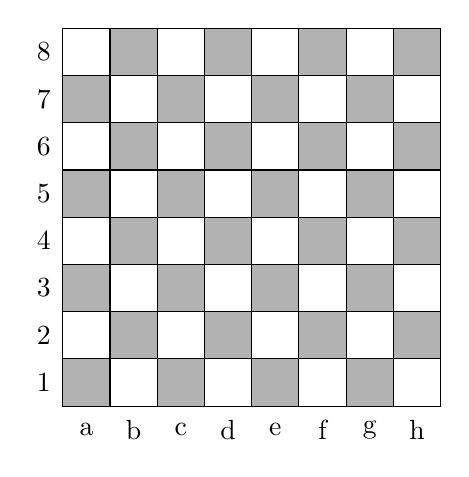
\begin{tikzpicture}[x=6mm,y=6mm]
\draw[fill=black!30,even odd rule] (0,0)
foreach \n in {1,2,3,4} { -- ++ (8,0) -- ++ (0,1) -- ++ (-8,0) -- ++ (0,1) } -- (8,8)

foreach \n in {1,2,3,4} { -- ++ (0,-8) -- ++ (-1,0) -- ++ (0,8) -- ++ (-1,0) } -- cycle

foreach[count=\n] \m in {a,b,...,h} { (-0.4,\n-0.5) node {\n} (\n-0.5,-0.5) node {\m} };

\end{tikzpicture}
\end{center}

Eine Lösung des Springerproblems mit Startfeld \j{h1} sieht wie folgt
aus. Die Felder sind in ihrer Besuchsreihenfolge durchnummeriert. Der
Springer bewegt sich also von \j{h1} nach \j{f2}, dann von \j{f2} nach
\j{h3} usw.

\begin{center}
\begin{tabular}{cccccccc}
41&10&29&26&49&12&31&16\\
28&25&40&11&30&15&50&13\\
9&42&27&56&61&48&17&32\\
24&39&58&47&64&53&14&51\\
43&8&55&62&57&60&33&18\\
38&23&46&59&54&63&52&3\\
7&44&21&36&5&2&19&34\\
22&37&6&45&20&35&4&1\\
\end{tabular}
\end{center}

\noindent
Formulieren Sie einen rekursiven Algorithmus zur Lösung des
Springerproblems von einem vorgegebenen Startfeld aus. Es sollen dabei
alle möglichen Lösungen des Springerproblems gefunden werden. Die
Lösungen sollen durch Backtracking gefunden werden. Hierbei werden alle
möglichen Teilrouten systematisch durchprobiert, und Teilrouten, die
nicht zu einer Lösung des Springerproblems führen können, werden nicht
weiterverfolgt. Dies ist durch rekursiven Aufruf einer Lösungsfunktion
\j{huepf(z, y, z)} zu realisieren, wobei

\begin{itemize}

\item \j{x} und \j{y} die Koordinaten des als nächstes anzuspringenden
Feldes sind, und

\item \j{z} die aktuelle Rekursionstiefe enthält. Wenn die
Rekursionstiefe $64$ erreicht und das betreffende Feld noch unbesucht ist,
ist eine Lösung des Springerproblems gefunden.
\end{itemize}

Der initiale Aufruf Ihres Algorithmus kann beispielsweise über den
Aufruf

\begin{center}
\j{huepf(1, 8, 1)}
\end{center}

erfolgen.

Wählen Sie geeignete Datenstrukturen zur Verwaltung der unbesuchten
Felder und zum Speichern gefundener (Teil)Lösungen. Der Algorithmus soll
eine gefundene Lösung in der oben angegebenen Form ausdrucken, also als
Matrix mit der Besuchsreihenfolge pro Feld.

\begin{bAntwort}
\bJavaExamen{46115}{2018}{09}{Springerproblem}
\end{bAntwort}
\end{document}
